\documentclass[preprint,12pt,a4paper]{elsarticle}

\usepackage{amssymb}
\usepackage{amsmath}
\usepackage{graphicx}
\usepackage{booktabs}
\usepackage{hyperref}
\usepackage{listings}
\usepackage{xcolor}
\usepackage{tikz}
\usetikzlibrary{arrows.meta,positioning,shapes.geometric,fit,backgrounds,calc}

\lstset{
  language=Python,
  basicstyle=\ttfamily\footnotesize,
  keywordstyle=\color{blue},
  commentstyle=\color{gray},
  stringstyle=\color{red!70!black},
  frame=single,
  breaklines=true,
  captionpos=b,
}

\journal{SoftwareX}

\begin{document}

\begin{frontmatter}

\title{\texttt{weatherisk}: A Python Package for Spatial Clustering
  of Climate Extremes via Max-Stable Processes}

\author[awi,uni]{Widad Kchikach\corref{cor1}}
\ead{widad.kchikach@awi.de}
\cortext[cor1]{Corresponding author}

\author[uni]{Thorsten Dickhaus}
\author[awi,uni]{Gerrit Lohmann}

\address[awi]{Alfred Wegener Institute Helmholtz Centre for Polar
  and Marine Research, Bremerhaven, Germany}
\address[uni]{University of Bremen, Bremen, Germany}

\begin{abstract}
We present \texttt{weatherisk}, an open-source Python package that
identifies regions of similar extreme-weather behaviour by clustering
gridded climate data.  Starting from daily observations, the software
extracts annual maxima, fits extreme-value distributions, and models
the spatial dependence of extremes using max-stable processes.  It
then estimates local anisotropy parameters at every grid cell and
groups cells into clusters where the dependence structure is
homogeneous.  Two complementary clustering methods are provided:
one based on the overlap of locally estimated anisotropy ellipses
(LEC) and one based on pairwise extremal dependence coefficients
(EDC).  The package faithfully reproduces an established R-based
pipeline in Python, verified by 50 automated cross-validation tests,
and adds a command-line interface, scalable estimation strategies,
and real-data pipelines for NOAA CPC climate reanalysis products.
\end{abstract}

\begin{keyword}
spatial extremes \sep max-stable process \sep
spatial clustering \sep spatial dependence \sep Python \sep
hierarchical clustering
\end{keyword}

\end{frontmatter}

%% ============================================================
\section*{Metadata}
\label{sec:metadata}
%% ============================================================

\begin{table}[!h]
\begin{tabular}{|l|p{6.5cm}|p{6.5cm}|}
\hline
\textbf{Nr.} & \textbf{Code metadata description} & \textbf{Metadata} \\
\hline
C1 & Current code version & v0.1.0 \\
\hline
C2 & Permanent link to code/repository &
  \url{https://github.com/widad-the-physicist/weatherisk} \\
\hline
C3 & Permanent link to Reproducible Capsule &
  \url{https://doi.org/xx.xxxx/zenodo.xxxxxxx} (to be minted) \\
\hline
C4 & Legal Code License & MIT \\
\hline
C5 & Code versioning system used & git \\
\hline
C6 & Software code languages, tools, and services used & Python~3 \\
\hline
C7 & Compilation requirements, operating environments
  \& dependencies &
  Python~$\geq$3.10; NumPy; SciPy; pandas; matplotlib;
  Click; xarray; netCDF4; scikit-learn; Cartopy \\
\hline
C8 & Link to developer documentation &
  \url{https://github.com/widad-the-physicist/weatherisk} \\
\hline
C9 & Support email for questions & widad.kchikach@awi.de \\
\hline
\end{tabular}
\caption{Code metadata (mandatory).}
\label{tab:metadata}
\end{table}


%% ============================================================
\section{Motivation and significance}
\label{sec:motivation}
%% ============================================================

Extreme weather events such as heavy precipitation or heat waves
rarely affect a single location in isolation; they tend to strike
entire regions simultaneously~[1].  Quantifying \emph{where} such
events tend to co-occur is essential for regional risk assessment,
reinsurance modelling, and infrastructure planning.  When the spatial
extent of extremes is neglected, the aggregate impact of a
widespread event can be severely underestimated.

\emph{Max-stable processes} offer a principled framework for
modelling the joint tail behaviour of spatially distributed
extremes~[2,3].  Following the approach of Contzen et al.~[4],
one can fit location-specific anisotropy parameters that describe
the strength and directional orientation of spatial dependence at
each grid point.  Grid points whose estimated parameters are
similar can then be grouped into \emph{clusters}---contiguous
regions where the dependence structure is approximately
homogeneous.

An R-based pipeline for this type of spatial clustering was developed
by Contzen et al.~[4].  It simulates max-stable processes,
estimates local anisotropy parameters through pairwise composite
likelihood, builds a dissimilarity matrix from ellipse overlaps, and
applies hierarchical clustering.  However, the original
implementation is split across several R scripts orchestrated by
SLURM shell files, making it difficult to install, test, or extend.

\texttt{weatherisk} solves this problem by re-implementing the full
pipeline in a single Python package that can be installed with
\texttt{pip install}.  It faithfully reproduces every step of the
original R code---verified by 50 automated tests that compare
key intermediate results to within a tolerance of $10^{-10}$---and
adds several
practical features:
\begin{itemize}
\item a command-line interface for running the pipeline with a single
  command;
\item extreme-value pre-processing (fitting distributions to annual
  maxima) so that raw climate data can be used directly;
\item a real-data pipeline that reads NOAA CPC daily NetCDF files and
  produces publication-ready cluster maps; and
\item a scalable strategy that allows global grids with hundreds of
  thousands of cells to be processed on standard HPC hardware.
\end{itemize}

To our knowledge, no existing Python package offers this combination
of max-stable simulation, local composite-likelihood estimation, and
ellipse-based spatial clustering.  Packages such as
\texttt{pyextremes}~[5] and
\texttt{scikit-extremes}\footnote{\url{https://github.com/kikocorreoso/scikit-extremes}}
focus on univariate extreme-value analysis; the R package
\texttt{SpatialExtremes}~[6] provides max-stable simulation but
not the clustering pipeline.

%% ============================================================
\section{Software description}
\label{sec:description}
%% ============================================================

\subsection{Software architecture}
\label{sec:architecture}

\texttt{weatherisk} is a pip-installable Python package organised
into 18~modules and a CLI entry point.  Figure~\ref{fig:workflow}
shows the overall workflow.

The processing pipeline consists of five stages:
\begin{enumerate}
\item \textbf{Data preparation.}
  Raw daily climate data (NetCDF) are loaded, annual block maxima are
  extracted, and extreme-value distributions (GEV) are fitted at each
  grid cell.  The fitted values are transformed to unit
  Fr\'{e}chet margins~[2] so that spatial dependence can be compared
  across locations.
\item \textbf{Simulation} (for validation on synthetic data).
  Non-stationary max-stable processes are generated on a regular grid
  with known parameters, following the spectral
  representation of Schlather~[7].
\item \textbf{Local estimation.}
  At each grid cell, the three anisotropy parameters---two semi-axis
  lengths and a rotation angle---are estimated by maximising a
  pairwise composite likelihood over neighbouring pairs, following
  the approach of Padoan et al.~[3].  Multiple random starting
  points are used to mitigate local optima~[4].  Estimates are
  then spatially smoothed.
\item \textbf{Clustering.}
  A pairwise dissimilarity matrix is computed from the estimated
  parameters, and hierarchical agglomerative clustering groups the
  grid cells into regions.  Two dissimilarity measures are available:
  ellipse-overlap (LEC) and madogram-based extremal coefficients
  (EDC, following Saunders et al.~[8]).
\item \textbf{Refinement.}
  Within each cluster, the dependence parameters are re-estimated
  using all data from the cluster's grid cells, and the
  goodness-of-fit of each method is assessed.
\end{enumerate}

\begin{figure}[ht]
\centering
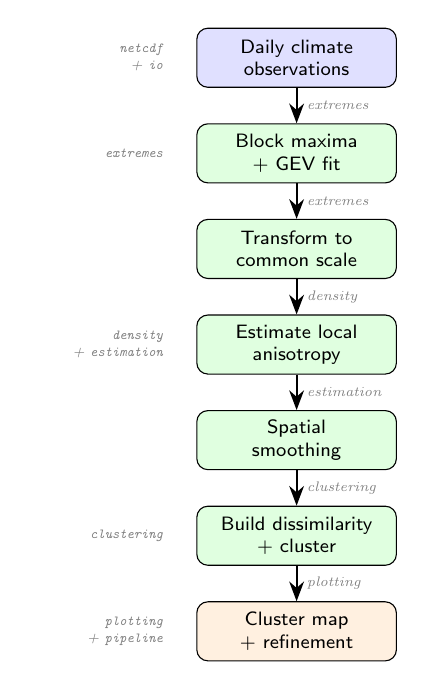
\begin{tikzpicture}[
  box/.style={draw, rounded corners=4pt, minimum width=2.4cm,
    minimum height=0.75cm, font=\sffamily\scriptsize,
    align=center, text width=2.3cm},
  data/.style={box, fill=blue!12},
  proc/.style={box, fill=green!12},
  outbox/.style={box, fill=orange!12},
  arr/.style={-{Stealth[length=2.5mm]}, thick},
  note/.style={font=\itshape\tiny, text=gray},
  node distance=0.45cm,
]

\node[data] (raw) {Daily climate\\observations};
\node[proc, below=of raw] (bm)
  {Block maxima\\+ GEV fit};
\node[proc, below=of bm] (frech)
  {Transform to\\common scale};
\node[proc, below=of frech] (mle)
  {Estimate local\\anisotropy};
\node[proc, below=of mle] (smooth)
  {Spatial\\smoothing};
\node[proc, below=of smooth] (clust)
  {Build dissimilarity\\+ cluster};
\node[outbox, below=of clust] (out)
  {Cluster map\\+ refinement};

\draw[arr] (raw) -- (bm)
  node[midway, right, note] {extremes};
\draw[arr] (bm) -- (frech)
  node[midway, right, note] {extremes};
\draw[arr] (frech) -- (mle)
  node[midway, right, note] {density};
\draw[arr] (mle) -- (smooth)
  node[midway, right, note] {estimation};
\draw[arr] (smooth) -- (clust)
  node[midway, right, note] {clustering};
\draw[arr] (clust) -- (out)
  node[midway, right, note] {plotting};

% Right-side annotation: module names
\node[note, left=0.3cm of raw, text width=1.6cm, align=right]
  {\texttt{netcdf}\\+ \texttt{io}};
\node[note, left=0.3cm of bm, text width=1.6cm, align=right]
  {\texttt{extremes}};
\node[note, left=0.3cm of mle, text width=1.6cm, align=right]
  {\texttt{density}\\+ \texttt{estimation}};
\node[note, left=0.3cm of clust, text width=1.6cm, align=right]
  {\texttt{clustering}};
\node[note, left=0.3cm of out, text width=1.6cm, align=right]
  {\texttt{plotting}\\+ \texttt{pipeline}};

\end{tikzpicture}
\caption{Processing pipeline of \texttt{weatherisk}.
  Boxes show the main stages; labels on the right indicate
  the module responsible; labels on the left show the corresponding
  Python module names.}
\label{fig:workflow}
\end{figure}

\subsection{Software functionalities}
\label{sec:functionalities}

\paragraph{Covariance modelling (\texttt{covariance}).}
This module computes the anisotropic covariance between any two
grid cells, given their semi-axis lengths and rotation angle.
It supports both the stationary case (constant parameters
everywhere) and the non-stationary case (parameters vary in
space), as well as the conversion between covariance values and
extremal dependence coefficients.

\paragraph{Simulation (\texttt{simulation}).}
Generates synthetic max-stable realisations with spatially
varying anisotropy.  This is used to validate the clustering
method on data where the true underlying structure is known.

\paragraph{Estimation (\texttt{density}, \texttt{estimation}).}
Estimates the three local parameters at each grid cell by fitting
the pairwise dependence model to all nearby pairs.  Multiple
random starting points are used to avoid poor local optima.
Results are spatially smoothed, and circular wrapping is
applied to the rotation angle.

\paragraph{Clustering (\texttt{clustering}).}
Computes the full pairwise dissimilarity matrix and applies
average-linkage hierarchical clustering.  The number of clusters
is determined automatically by a quantile threshold on the
dendrogram merge heights.  Two dissimilarity measures are
implemented:
\begin{itemize}
\item \textbf{LEC} (Local Estimate Clustering): based on the
  Jaccard-like overlap of the anisotropy ellipses;
\item \textbf{EDC} (Extremal Dependence Clustering, following
  the terminology of Saunders et al.~[8]): based on
  rank-estimated pairwise extremal coefficients~[8,9].
\end{itemize}

\paragraph{Real-data support (\texttt{netcdf}, \texttt{extremes}).}
Reads NOAA CPC daily precipitation and temperature files,
extracts annual block maxima, fits GEV distributions, and
transforms to unit Fr\'{e}chet margins for dependence modelling.

\paragraph{Scalability (\texttt{scalable}).}
For large grids, local estimation runs at full resolution in
parallel, but clustering operates on a coarsened grid that fits
in memory.  Labels are then propagated back to the fine grid
and refined.  Intermediate results are checkpointed as NumPy
binary files, so that long-running jobs can be resumed after
interruption.

\subsection{Computational performance}
\label{sec:performance}

The two most expensive steps in the pipeline are (i)~building the
pairwise dissimilarity matrix, which must compare every pair of
grid cells ($O(n^2)$ comparisons for $n$~cells), and (ii)~the
local parameter estimation, which solves one optimisation problem
per grid cell.  In the original R~code both steps are implemented
with nested \texttt{for}-style loops that process one pair (or one
cell) at a time, calling a general-purpose matrix-inversion routine
for each pair.  This approach is simple to write but slow, because
every iteration carries the overhead of the R~interpreter and of
general-purpose linear-algebra functions that are more costly than
necessary for the small $2\times 2$ matrices involved.

\texttt{weatherisk} replaces these one-at-a-time loops with four
strategies that process many cells or pairs simultaneously:

\begin{enumerate}
\item \textbf{Batch covariance computation.}
  Instead of computing the covariance between one pair of cells at
  a time, the package builds the entire $n \times n$ covariance
  table in one operation using NumPy array arithmetic.  Because each
  local covariance matrix is only $2\times 2$, its inverse can be
  written as a simple closed-form expression (swap the diagonal,
  negate the off-diagonal, divide by the determinant), avoiding the
  cost of calling a general-purpose matrix solver for every pair.

\item \textbf{Pre-drawn ellipse overlap.}
  The LEC dissimilarity between two grid cells is the overlap area
  of their estimated anisotropy ellipses.  Rather than re-drawing
  both ellipses every time a pair is compared, each ellipse is
  drawn \emph{once} onto a shared pixel image.  The overlap between
  any two ellipses then reduces to counting the pixels that both
  images share---a fast Boolean operation.  Pairs are processed in
  batches (default 256~rows at a time) to keep memory usage
  manageable.

\item \textbf{Fast pairwise distance computation for EDC.}
  The EDC method measures how similar two grid cells are by
  comparing the ranks of their extreme values (the so-called
  madogram).  \texttt{weatherisk} delegates this
  rank-difference calculation to \texttt{scipy.spatial.distance.cdist},
  a routine implemented in compiled C~code that processes all
  pairs in a single call, rather than looping over them in
  Python.  The initial ranking of the data also uses an efficient
  sort-based algorithm ($O(n \log n)$) instead of the slower
  pairwise-comparison approach ($O(n^2)$) used in the R~code.

\item \textbf{Parallel local estimation.}
  Each grid cell's parameters are estimated independently, which
  makes this step straightforward to parallelise.  The package
  distributes the estimation tasks across all available CPU cores
  using Python's \texttt{multiprocessing} library.  The large
  shared data arrays are set up once when the worker processes
  start, so that they do not need to be copied for every task.
  When only a single core is used, the parallelisation layer is
  skipped entirely to avoid unnecessary overhead.
\end{enumerate}

Table~\ref{tab:benchmark} in Appendix~\ref{app:benchmark} reports
wall-clock timings that illustrate the effect of these optimisations
on a $21\times 21$ synthetic grid (441~cells, 10~realisations) run
on an Apple~M2 processor.

\paragraph{Command-line interface (\texttt{cli}).}
A single entry point exposes the main pipeline flows:
\begin{lstlisting}[numbers=none]
$ weatherisk validate --params stripes \
    --resolution 10 --n-sim 20 --seed 42
$ weatherisk maps --variable precip
\end{lstlisting}

%% ============================================================
\section{Illustrative examples}
\label{sec:examples}
%% ============================================================

We demonstrate \texttt{weatherisk} with three examples: one on
synthetic data and two on real precipitation observations.

\subsection{Example~1: Recovering known structure from
  synthetic data}
\label{sec:ex-synthetic}

In this example, we simulate max-stable data on a 51$\times$51 grid
where the semi-major axis $b$ increases linearly from left to right,
creating vertical ``stripe'' regions.  The pipeline should recover
these stripes from the simulated data alone.

\begin{lstlisting}[caption={Running the stripes validation.},
  label=lst:validate]
from weatherisk.parameters import get_preset
from weatherisk.pipeline import run_pipeline

result = run_pipeline(
    resolution=51, n_sim=20,
    preset="stripes", seed=42,
)
\end{lstlisting}

Figure~\ref{fig:stripes} shows the result.  Panel~(a) displays the
EDC clusters ($k_{\text{edc}} = 7$), panel~(b) the LEC clusters
($k_{\text{lec}} = 5$), and panel~(c) the true parameter field.
The true semi-major axis~$b$ increases smoothly from left to right
(panel~c), producing a continuous gradient from dark blue ($b
\approx 0$) on the left to light shading ($b \approx 5$) on the
right.  The EDC method (panel~a) uses seven clusters and captures
the overall left-to-right trend, but its boundaries are irregular:
some clusters extend horizontally across the domain, and the
transitions between adjacent regions do not follow the vertical
orientation of the true gradient.  The LEC method (panel~b), by
contrast, uses only five clusters yet produces boundaries that are
predominantly vertical, closely tracking the true transitions in
the parameter field.  The estimated within-cluster~$b$ values in
the LEC map also progress monotonically from dark to light,
mirroring the ground truth more faithfully than the EDC partition.
This controlled experiment illustrates that the Python
implementation correctly recovers the known spatial structure,
consistent with the methodology of Contzen et al.~[4].  Formal
verification of numerical equivalence with the original R code
is provided by the 50~automated cross-validation tests described
in Section~\ref{sec:impact}.  The example also demonstrates the
advantage of ellipse-overlap dissimilarity for recovering
spatially structured anisotropy patterns.

\begin{figure*}[ht]
\centering
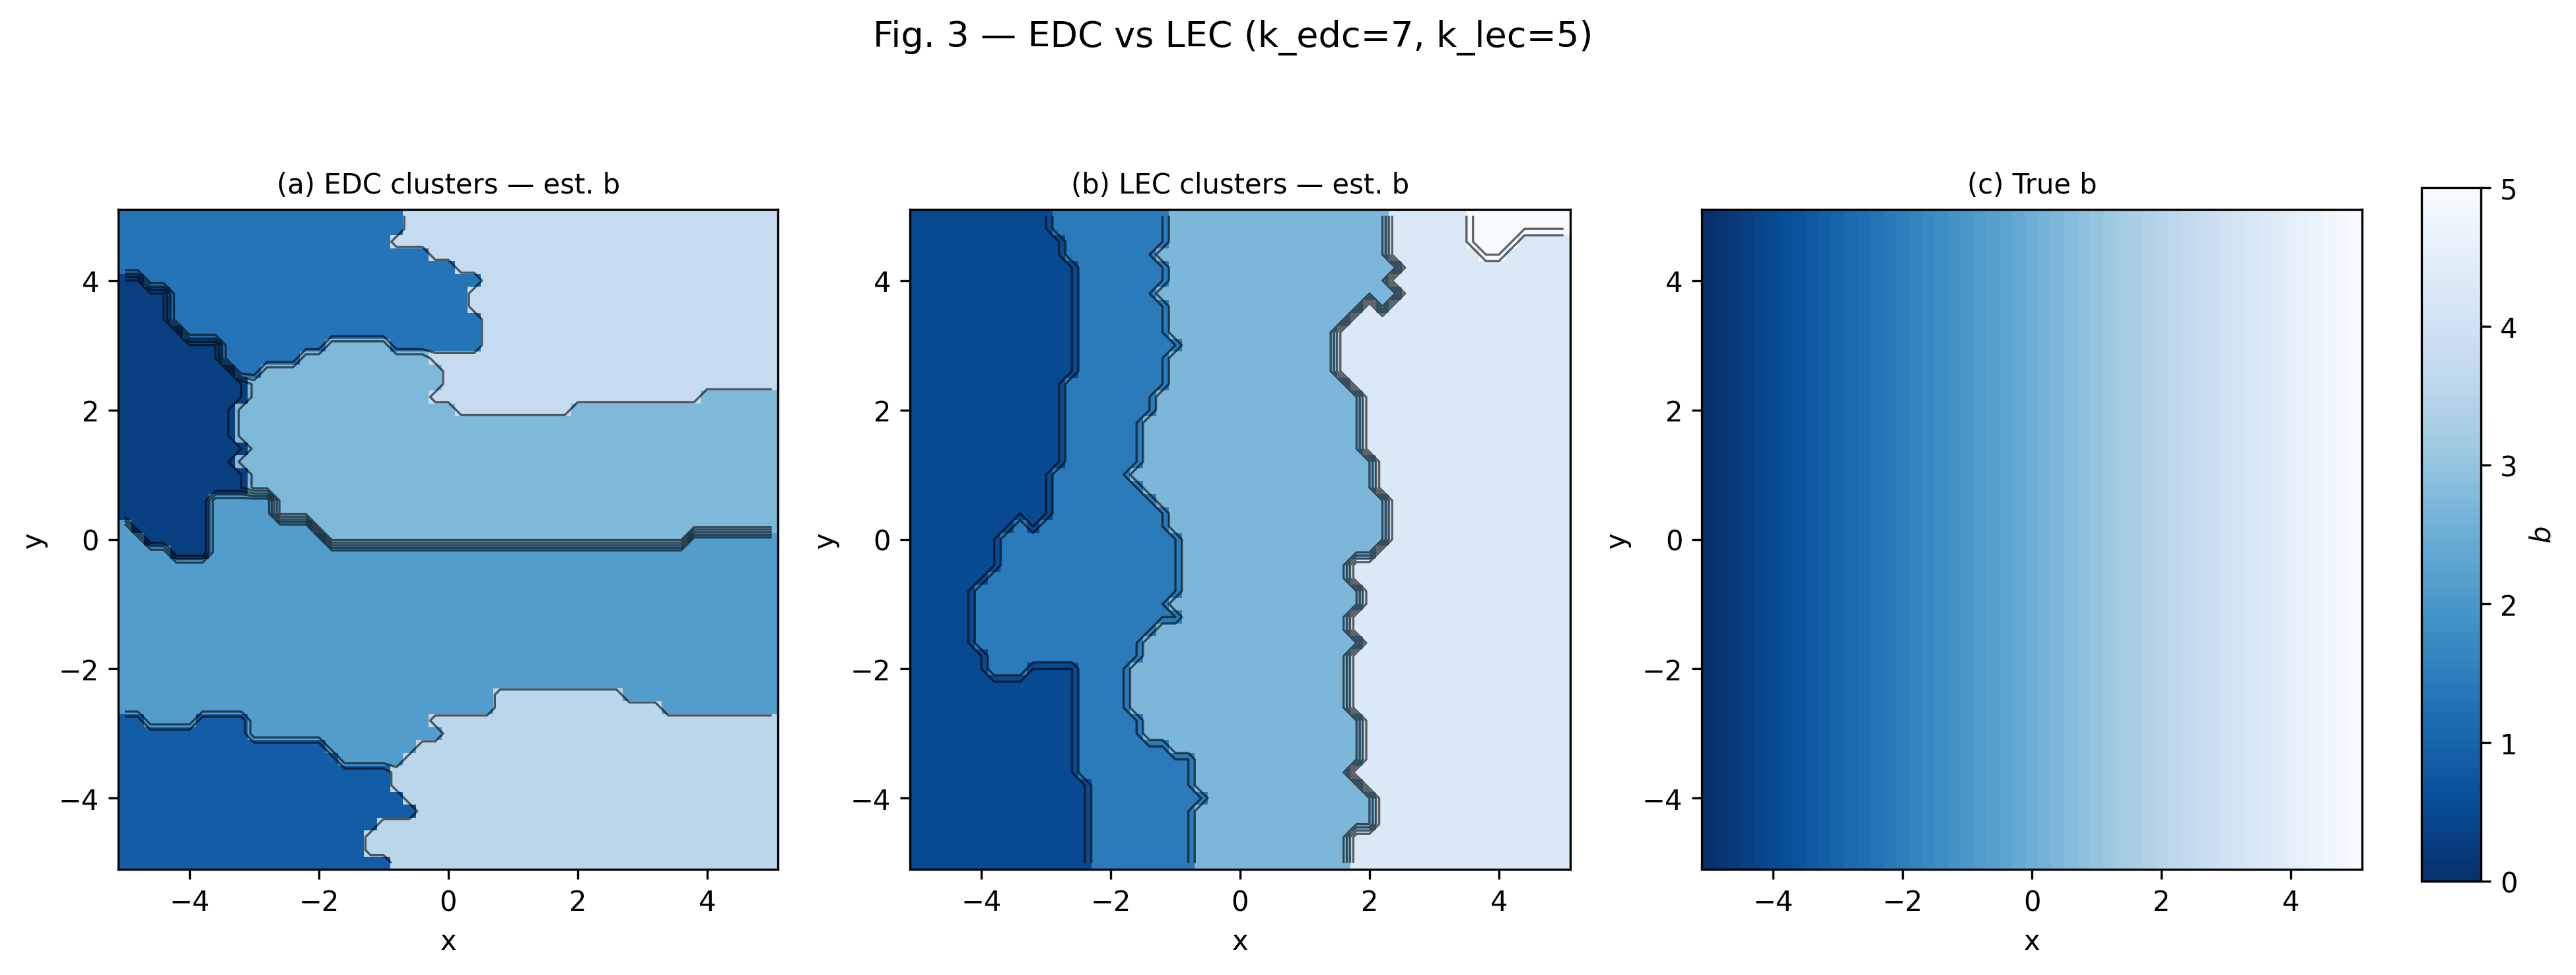
\includegraphics[width=0.95\textwidth]{figures/fig3_regenerated.png}
\caption{Synthetic validation on the ``stripes'' preset
  ($k_{\text{edc}} = 7$, $k_{\text{lec}} = 5$).
  (a)~EDC clusters coloured by estimated semi-major axis~$b$;
  (b)~LEC clusters coloured by estimated~$b$;
  (c)~true parameter field showing a smooth left-to-right
  gradient in~$b$ from 0 to~5.
  The LEC method recovers sharper, vertically aligned boundaries
  that closely match the ground truth, while the EDC method
  produces more irregular, horizontally extended partitions.}
\label{fig:stripes}
\end{figure*}

\subsection{Example~2: LEC clustering of precipitation extremes}
\label{sec:ex-lec}

We apply the full real-data pipeline to 20~years (2000--2019) of
NOAA CPC daily precipitation over a European--Middle Eastern domain
(30\textdegree--65\textdegree N, 5\textdegree--55\textdegree E),
coarsened to approximately 2\textdegree\ resolution (384~land
cells).

\begin{lstlisting}[caption={Running the CPC maps pipeline.},
  label=lst:maps]
$ weatherisk maps --variable precip
\end{lstlisting}

Figure~\ref{fig:lec-map} shows the resulting LEC cluster map.
The method uses the ellipse-overlap dissimilarity~$D_2$ and
identifies $k = 26$ clusters with a 30\%-quantile dendrogram
threshold.  The spatial pattern reveals physically coherent,
spatially contiguous regions.  Scandinavia and the Norwegian coast
form a large, dominant cluster (orange), indicating that
precipitation extremes across that region share a homogeneous
spatial dependence structure.  A second large cluster (light purple
and grey tones) covers much of the continental interior, spanning
from Eastern Europe through western Russia.  Smaller clusters pick
out climatically distinct sub-regions: the Mediterranean coastline,
the British Isles, the Alpine arc, and parts of the Middle East
each receive their own groupings.  Notably, the large majority of
clusters are spatially contiguous, meaning that grid cells
assigned to the same cluster tend to be geographical neighbours.
This is a characteristic strength of the ellipse-overlap
approach: because it compares the \emph{shape} and
\emph{orientation} of local anisotropy ellipses, neighbouring
cells whose dependence geometry is similar are naturally grouped
together, producing regions that often align with geographic
features such as coastlines and mountain ranges.
The full pipeline---data loading, GEV fitting, local estimation,
smoothing, clustering, and map generation---runs in approximately
100~seconds on an Apple~M2 laptop with 16\,GB RAM.

\begin{figure}[ht]
\centering
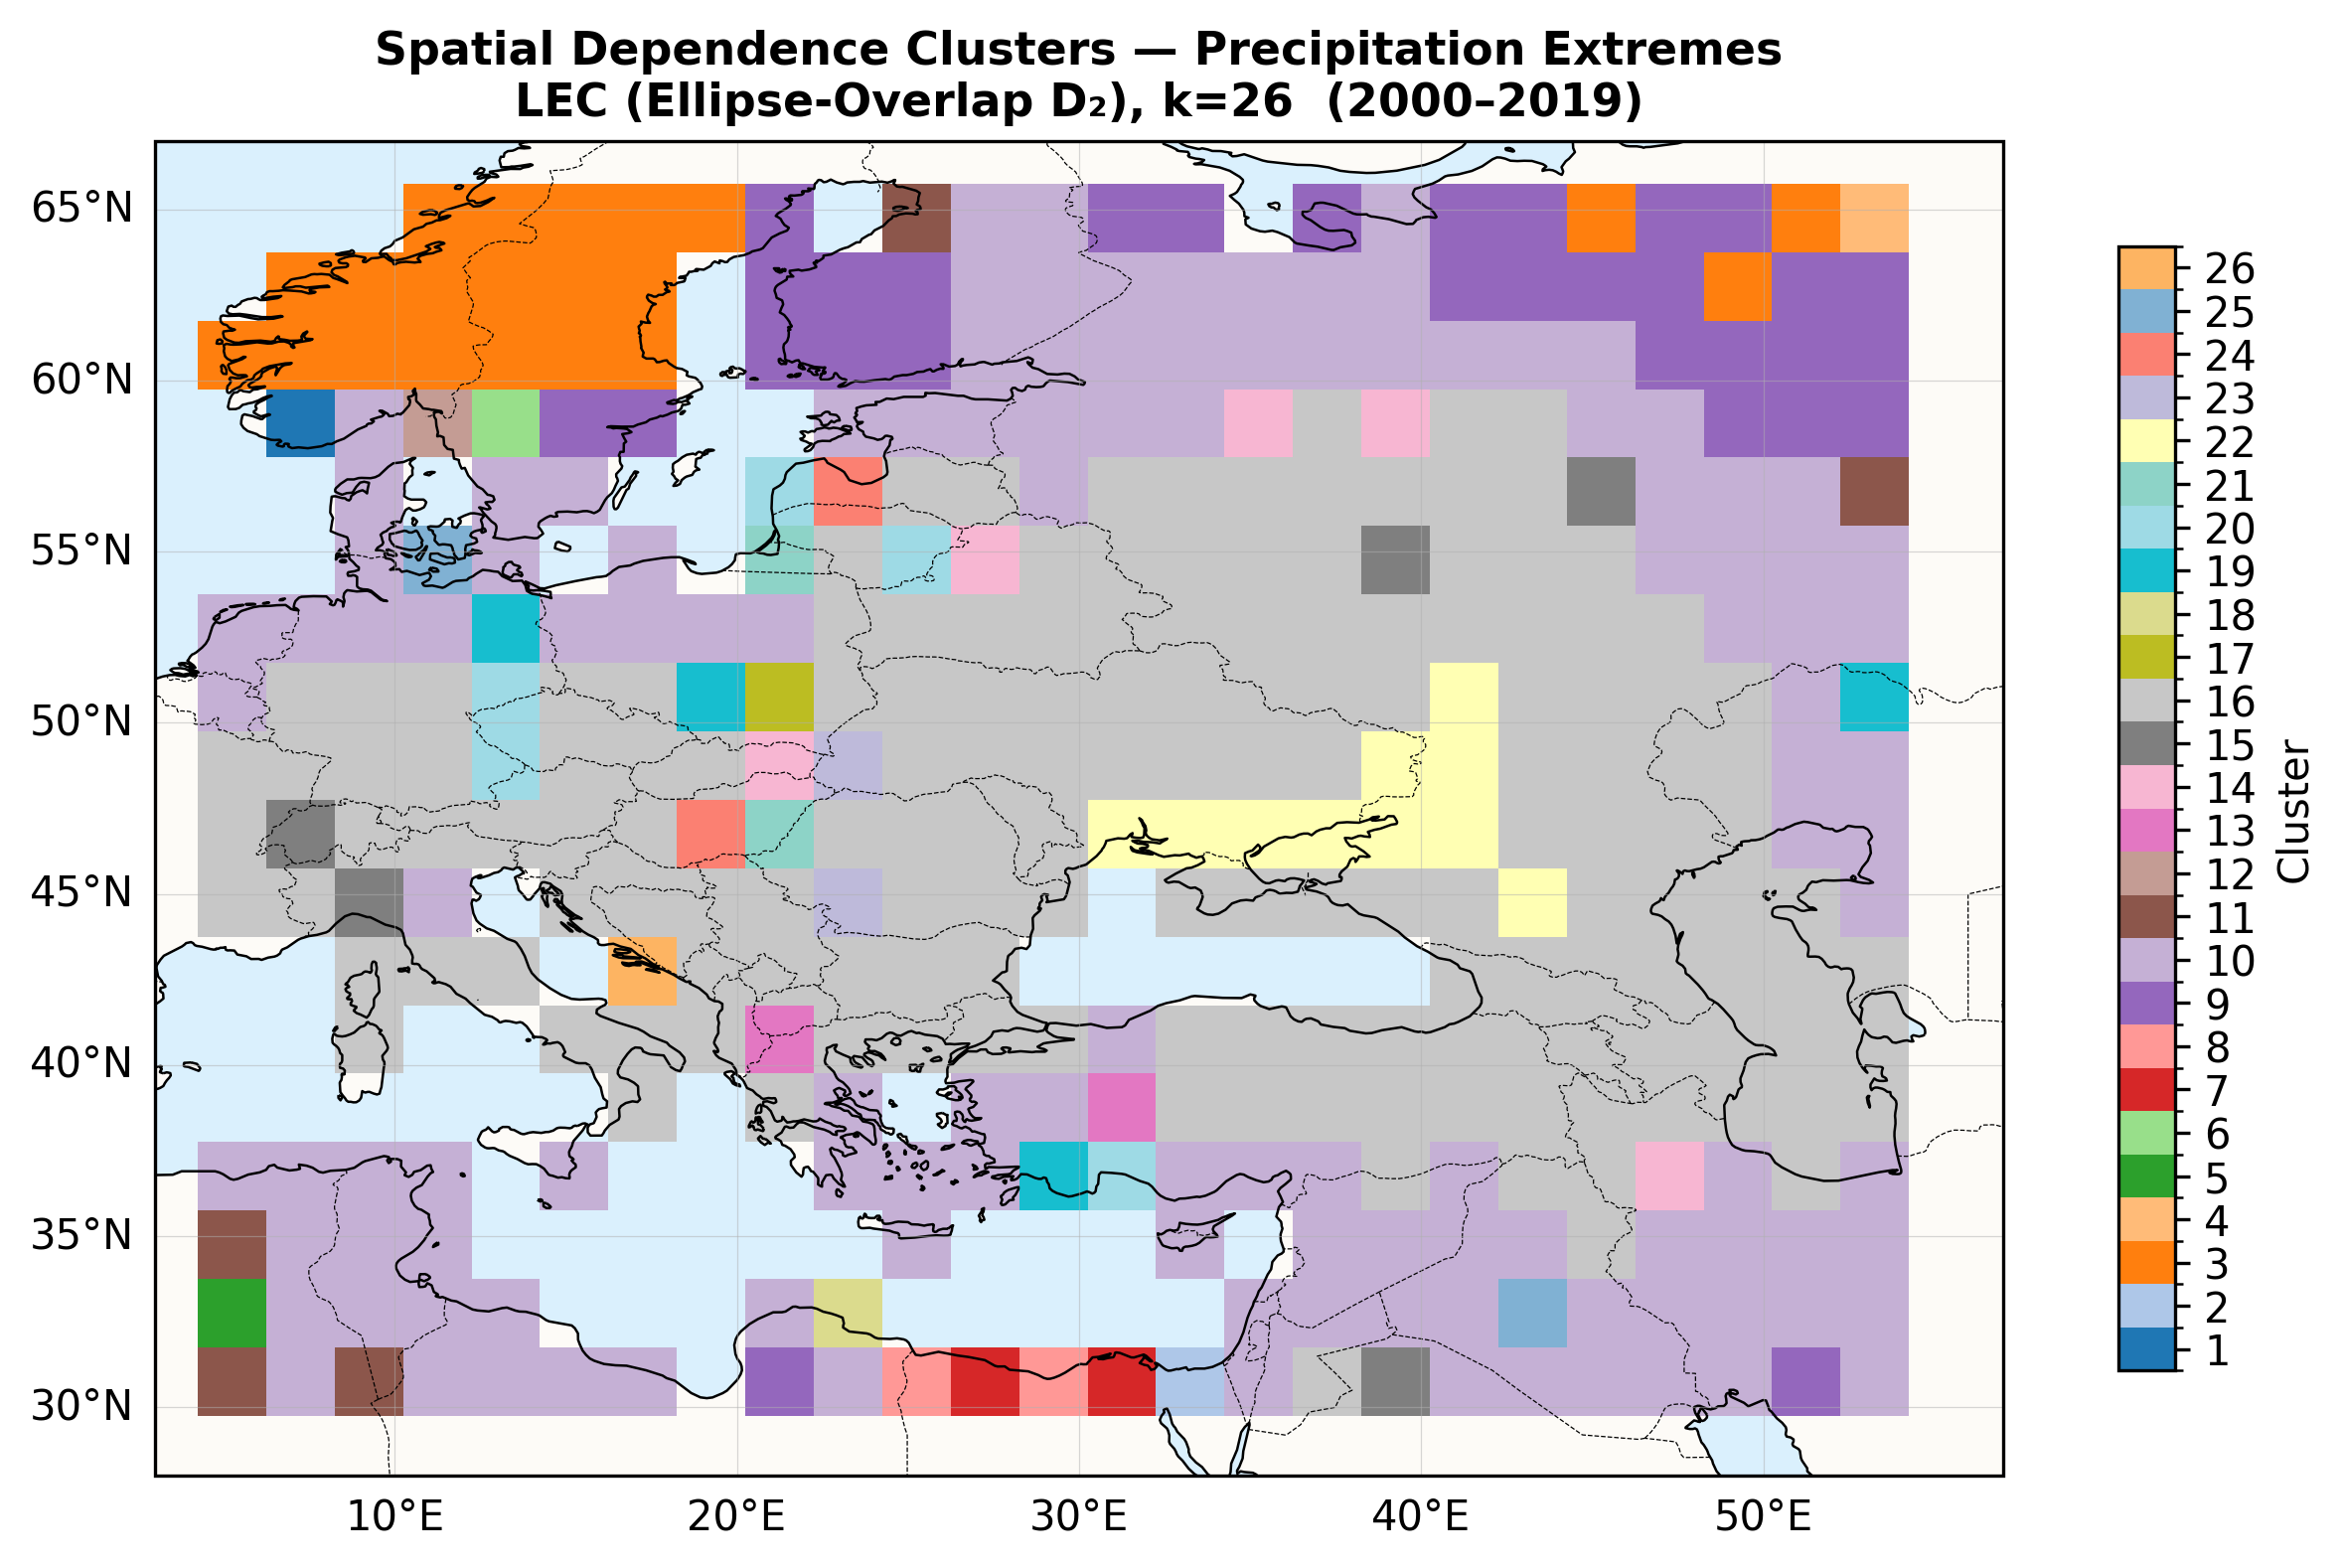
\includegraphics[width=0.95\columnwidth]{figures/lec_clusters_map.png}
\caption{LEC spatial dependence clusters for precipitation
  extremes using ellipse-overlap dissimilarity~$D_2$
  (2000--2019, $k = 26$).  Each colour identifies a region
  where extreme precipitation events share a similar spatial
  dependence structure.  The map is dominated by large,
  spatially contiguous clusters---Scandinavia (orange) and the
  continental interior (light purple/grey)---with smaller
  clusters picking out coastlines and mountain regions.}
\label{fig:lec-map}
\end{figure}

\subsection{Example~3: EDC clustering of precipitation extremes}
\label{sec:ex-edc}

For comparison, Figure~\ref{fig:edc-map} shows the EDC cluster map
produced from the same precipitation data.  The EDC method uses the
madogram-based extremal dependence coefficient~$D_1$~[8,9] rather
than locally estimated ellipse parameters and identifies $k = 18$
clusters.  Although $k = 18$ is smaller than the 26~clusters
obtained by LEC, the resulting map appears far more heterogeneous:
the same cluster colour is scattered across widely separated parts
of the domain, and very few clusters form large, spatially
contiguous blocks.  For instance, the pink cluster (cluster~8)
appears both in southern Turkey and in continental Poland, and the
green cluster (cluster~5) spans disparate cells from the Balkans to
the Caspian coast.  This spatial fragmentation is a direct
consequence of the madogram dissimilarity: the madogram measures
the rank-based tendency of two grid cells to jointly exceed high
thresholds, but it does not account for the directional shape
or orientation of the spatial dependence.  Two geographically
distant cells can therefore have a similar pairwise extremal
coefficient---and hence be grouped into the same cluster---without
sharing the same local anisotropy structure.

Together, the two methods provide complementary perspectives on
spatial dependence.  LEC preserves geographic coherence by
comparing the shape and orientation of locally estimated
anisotropy ellipses, producing large contiguous regions that
align with known climatic boundaries (Figure~\ref{fig:lec-map}).
EDC, by contrast, groups cells by the overall \emph{strength}
of extremal dependence regardless of spatial proximity, which
can reveal long-range similarities in dependence magnitude
that the ellipse-based method does not capture.

\begin{figure}[ht]
\centering
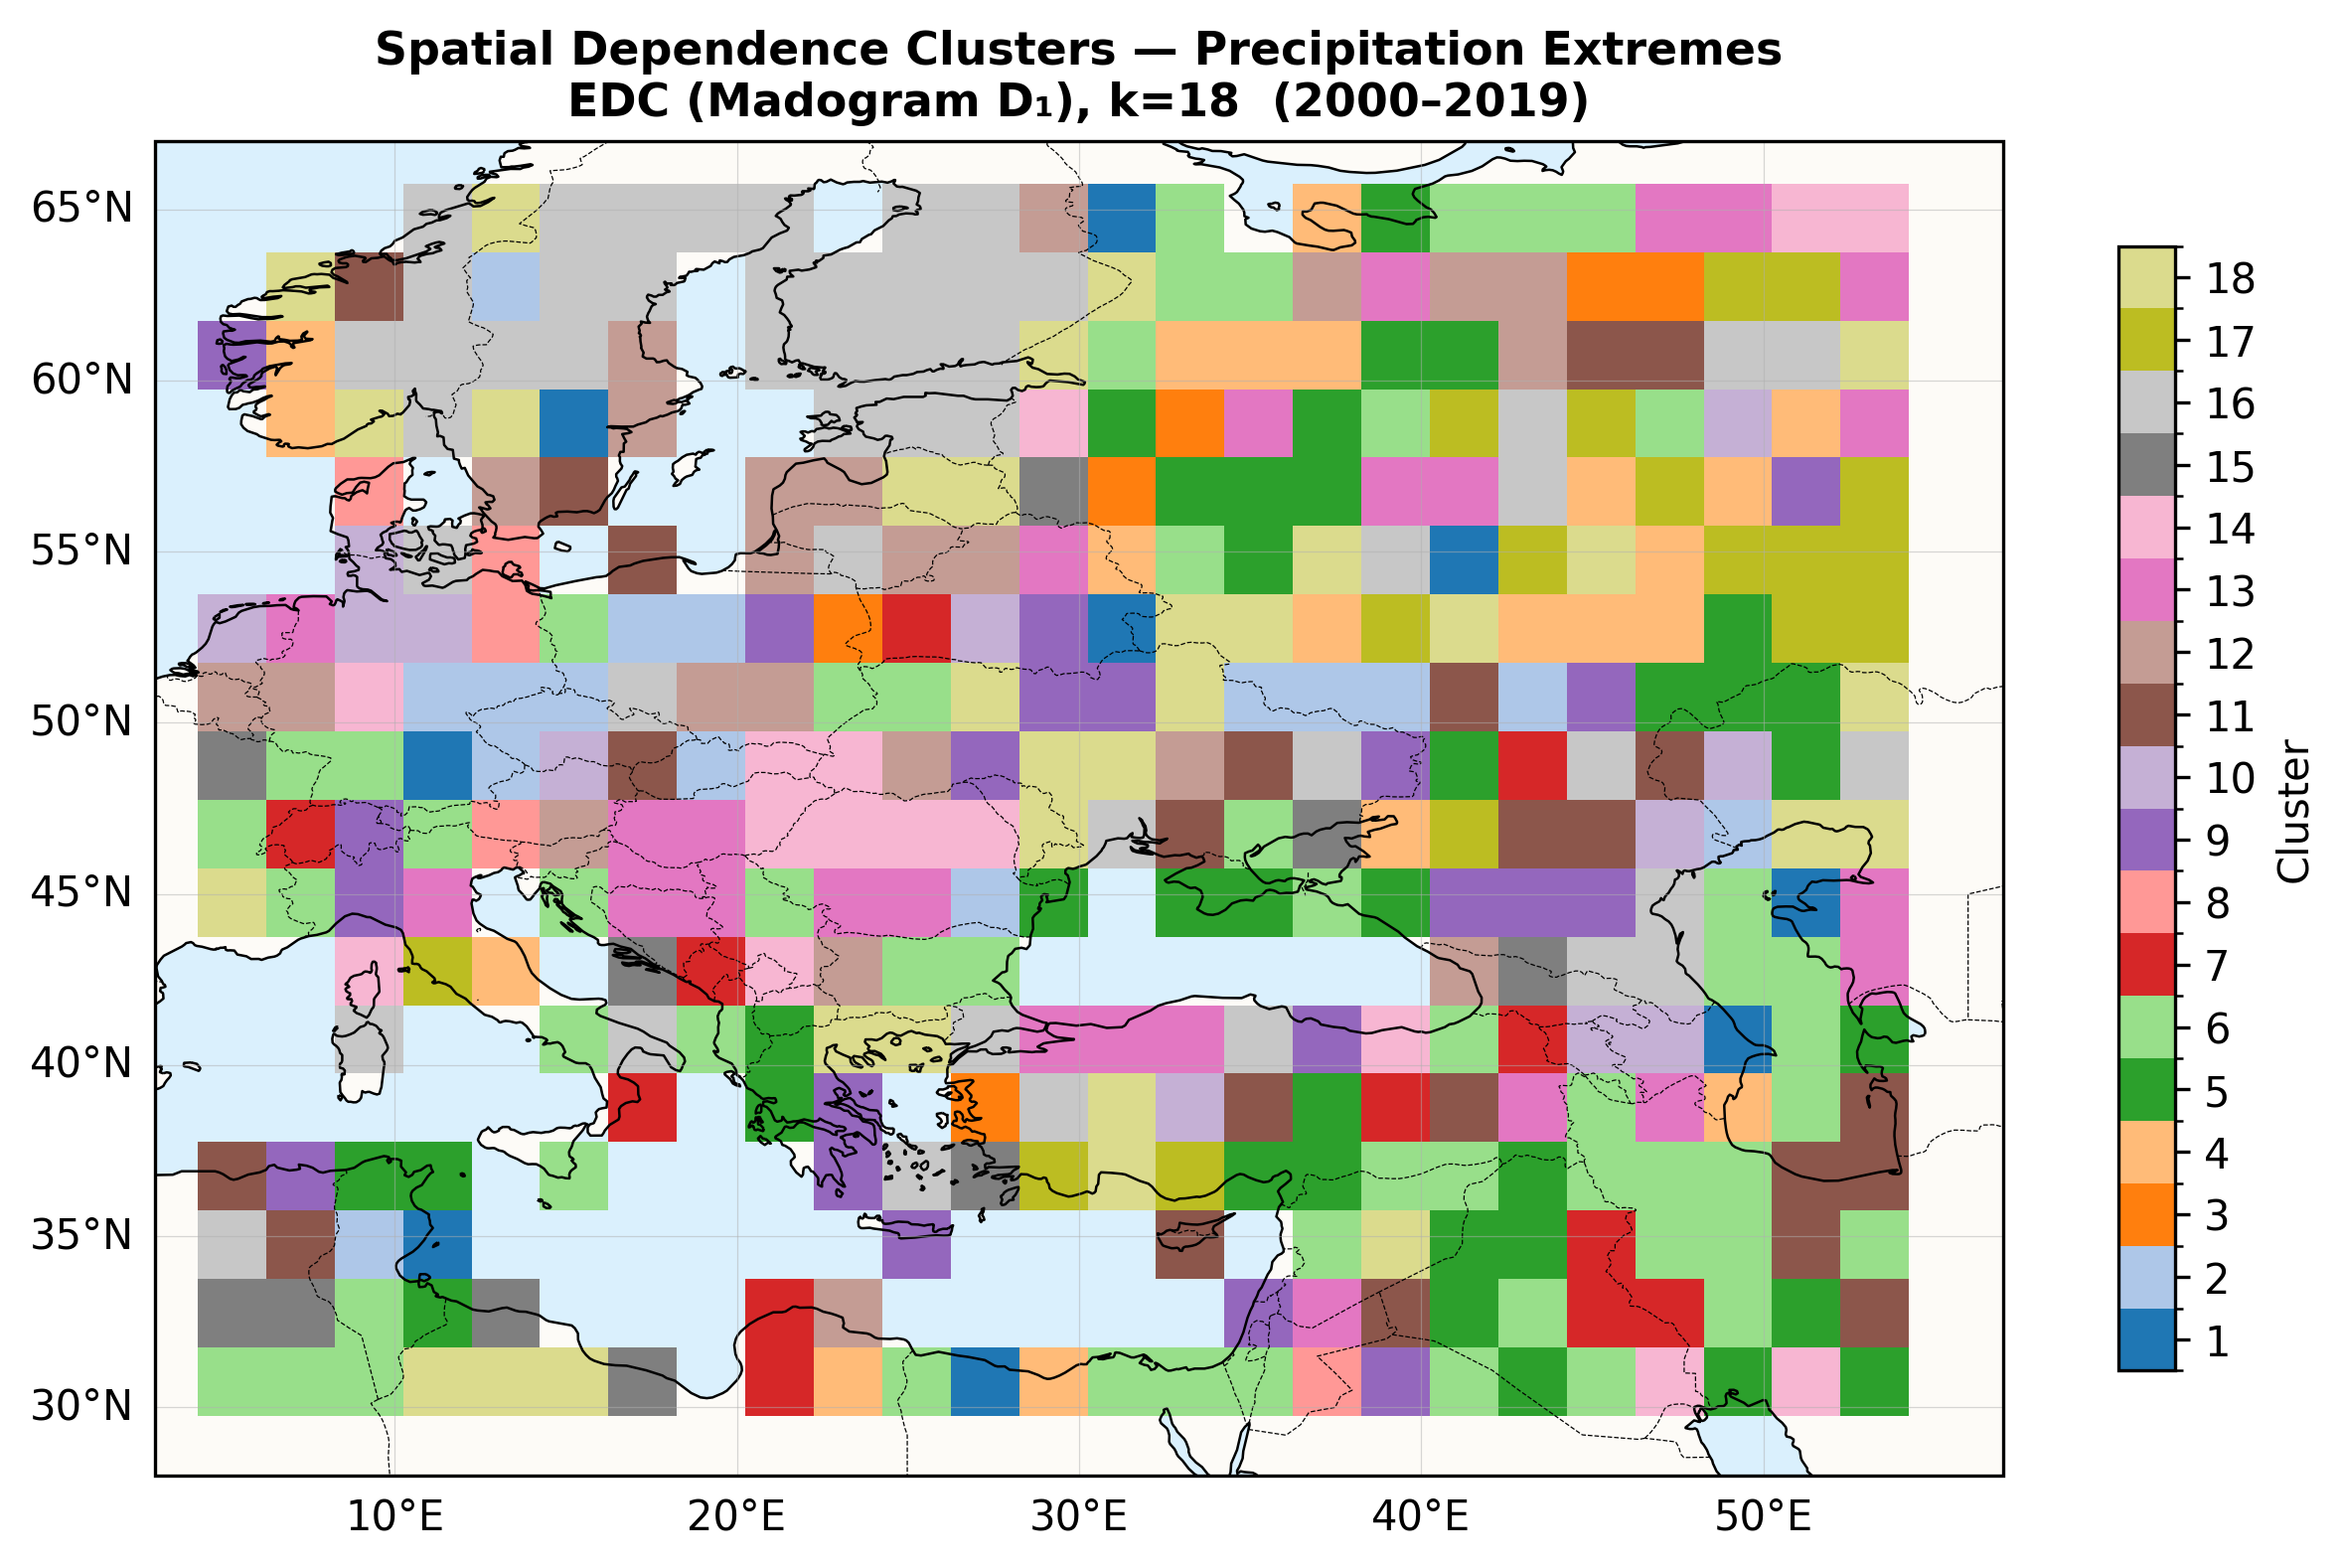
\includegraphics[width=0.95\columnwidth]{figures/edc_clusters_map.png}
\caption{EDC spatial dependence clusters for precipitation
  extremes using madogram-based dissimilarity~$D_1$
  (2000--2019, $k = 18$).  Despite using fewer clusters than
  LEC (Figure~\ref{fig:lec-map}), the EDC map is visibly more
  fragmented: the same cluster colour appears in widely
  separated locations across the domain, reflecting the
  rank-based, non-directional nature of the madogram
  dissimilarity.}
\label{fig:edc-map}
\end{figure}


%% ============================================================
\section{Impact}
\label{sec:impact}
%% ============================================================

\texttt{weatherisk} makes an established spatial-extreme clustering
methodology accessible as a standard Python package, removing
the barrier of multi-language R/Shell/SLURM workflows.

\paragraph{Reproducibility and correctness.}
The package includes over 100~automated tests.  Of these, 50 are
cross-validation tests that compare the Python output against
reference values produced by the original R~code at every stage of
the pipeline---from individual covariance values through to the
final cluster labels.  All comparisons pass with agreement to
at least ten decimal places.

Achieving this level of equivalence required several targeted
adjustments to account for differences between the two languages.
For example:
\begin{itemize}
\item R and Python store matrices in different internal orders
  (column-by-column vs.\ row-by-row), so the Python code explicitly
  matches R's ordering when converting matrices to flat arrays.
\item The rotation angle that describes ellipse orientation is
  periodic ($+90°$ equals $-90°$); both implementations must
  handle the wrap-around in the same way.
\item The log-likelihood is averaged over the number of grid-cell
  pairs before optimising, matching a convention in the R~code
  that affects the optimiser's convergence behaviour.
\end{itemize}
These and similar fixes ensure that published results based on
the R~code can be faithfully reproduced in Python.

\paragraph{New research directions.}
By providing a clean Python API and CLI, \texttt{weatherisk} lowers
the entry barrier for researchers who wish to apply spatial
clustering of extremes to new domains (e.g., wind speed, sea-level
pressure) or different datasets (e.g., ERA5, CMIP6 projections).


\paragraph{Education.}
The step-by-step pipeline design, the comprehensive test suite,
and the documented code examples (Appendix~\ref{app:code}) make
the package a practical resource for practitioners.  A Jupyter notebook tutorial
that walks through the full pipeline on synthetic data is
included in the repository.

\paragraph{Computational efficiency.}
The vectorisation and parallelisation strategies described in
Section~\ref{sec:performance} yield large practical speed-ups.
On a $21 \times 21$ synthetic grid (441~cells), the EDC
dissimilarity matrix is computed in 0.02\,s, and the full pipeline
including 8-core parallel estimation completes in under 1\,s
(see Appendix~\ref{app:benchmark}).  On the 384-cell real-data
domain, the end-to-end pipeline---data loading, GEV fitting,
local estimation, smoothing, clustering, and map generation---runs
in approximately 100\,s on an Apple~M2 laptop with 16\,GB RAM.
The coarse-grid proxy strategy in the \texttt{scalable} module is
designed to extend this approach to global grids with hundreds of
thousands of cells on standard HPC hardware.

%% ============================================================
\section{Conclusions}
\label{sec:conclusions}
%% ============================================================

We have presented \texttt{weatherisk}, a Python package that
implements the complete pipeline for spatial clustering of climate
extremes via max-stable processes.  The software consolidates a
fragmented R/Shell workflow into a single, tested, pip-installable
library.  Key contributions include:
\begin{enumerate}
\item a verified Python port of the entire clustering pipeline,
  proven equivalent to the original R code by 50~automated tests;
\item vectorised algorithms and multicore parallelism that
  achieve a 4.1$\times$ speed-up on 8~cores for the local
  estimation step, and complete both dissimilarity matrices in
  under 0.1\,s for 441~cells
  (Section~\ref{sec:performance}, Appendix~\ref{app:benchmark});
\item an automated real-data pipeline that reads NOAA CPC daily
  NetCDF files and handles the complete pre-processing chain:
  extracting annual block maxima, fitting extreme-value
  distributions, and transforming to a common statistical scale.
  The original R~code was designed for simulated data that is
  already on this scale, so it did not include any of these
  pre-processing steps; in \texttt{weatherisk} they are fully
  automated, allowing the user to go from raw climate observations
  to publication-ready cluster maps
  (Figures~\ref{fig:lec-map} and~\ref{fig:edc-map}) with a single
  command; and
\item scalable strategies for global grids.
\end{enumerate}
The modular design of the package makes it straightforward to
extend: planned additions include per-cluster risk metrics
(e.g.\ Value-at-Risk, Expected Shortfall), economic exposure
weighting, and support for climate model projections such as
CMIP6 scenarios.  \texttt{weatherisk} is available under the
MIT licence.

%% ============================================================
\section*{Acknowledgements}
%% ============================================================

to be completed after peer review

%% ============================================================
%% APPENDIX
%% ============================================================
\appendix

\section{Key code examples}
\label{app:code}

This appendix collects the main code snippets that a practitioner
needs to run the two pipeline flows shown in the paper.

\subsection{A.1\quad Synthetic validation (Flow~1)}

\begin{lstlisting}[caption={Complete synthetic validation
  workflow.}, label=lst:app-validate]
from weatherisk.parameters import get_preset
from weatherisk.simulation import simulate_non_stat
from weatherisk.grid import make_grid
from weatherisk.estimation import (
    calc_local_estimates,
    smooth_estimates,
    calc_estimates_in_clusters,
)
from weatherisk.clustering import (
    ellipse_dissimilarity,
    cluster_from_dissimilarity,
    saunders_clustering,
)
from weatherisk.plotting import plot_cluster_map

# 1. Load a parameter preset
p = get_preset("stripes")

# 2. Build a grid and simulate data
grid = make_grid(resolution=10)
data = simulate_non_stat(
    p.params, grid, n_sim=20,
    df=p.df, alpha=p.alpha, seed=42,
)

# 3. Estimate local anisotropy parameters
raw_est = calc_local_estimates(
    data, grid, df=p.df, alpha=p.alpha,
)
est = smooth_estimates(raw_est, grid)

# 4. Cluster by ellipse-overlap dissimilarity
D = ellipse_dissimilarity(est, grid)
clusters = cluster_from_dissimilarity(
    D, quantile_threshold=0.3,
)

# 5. Re-estimate within clusters
in_clust = calc_estimates_in_clusters(
    data, clusters, grid,
    df=p.df, alpha=p.alpha,
)

# 6. Plot
fig = plot_cluster_map(clusters, grid)
fig.savefig("lec_clusters.pdf")
\end{lstlisting}

\subsection{A.2\quad Real-data pipeline (Flow~2)}

\begin{lstlisting}[caption={CPC precipitation clustering via
  CLI.}, label=lst:app-cpc-cli]
# Run the full real-data pipeline from the
# command line (NetCDF files in data/netcdf/):
$ weatherisk maps --variable precip

# Or in Python:
from weatherisk.cpc_pipeline import run_cpc_maps
results = run_cpc_maps(variable="precip")
\end{lstlisting}

\subsection{A.3\quad Comparing LEC and EDC methods}

\begin{lstlisting}[caption={Running both clustering methods
  and comparing results.}, label=lst:app-compare]
from weatherisk.pipeline import run_pipeline
from weatherisk.plotting import (
    plot_cluster_map,
    plot_eici_comparison,
)

# Run full pipeline (includes both methods)
result = run_pipeline(
    resolution=10, n_sim=20,
    preset="stripes", seed=42,
)

# Access cluster labels
lec_labels = result["lec_clusters"]
edc_labels = result["edc_clusters"]

# Compare goodness-of-fit
fig = plot_eici_comparison(result)
fig.savefig("eici_comparison.pdf")
\end{lstlisting}

\section{Benchmark timings}
\label{app:benchmark}

Table~\ref{tab:benchmark} reports wall-clock timings for the Python
pipeline, measured on an Apple~M2 (8-core) laptop with 16\,GB RAM
running macOS~14 and Python~3.12.  The test case is a $21\times 21$
synthetic grid (441~cells) with 10~realisations, using the
``stripes'' parameter preset.  All times are medians of three runs.

The table shows how the total running time is distributed across
the main pipeline stages.  The most expensive step is the local
parameter estimation (MLE), which takes 3.10\,s when run on a
single core.  Distributing this work across 8~cores reduces it to
0.75\,s---a 4.1$\times$ speed-up.  The two dissimilarity matrices
(EDC and LEC) are both computed in well under 0.1\,s for 441~cells.
With parallel estimation enabled, the entire pipeline completes in
approximately 1\,s.

\begin{table}[ht]
\centering
\begin{tabular}{lr}
\toprule
\textbf{Pipeline stage} & \textbf{Time (s)} \\
\midrule
Simulation (441 cells, 10 realisations) & 0.17 \\
EDC dissimilarity matrix (441 cells) & 0.02 \\
LEC dissimilarity matrix (441 cells) & 0.06 \\
Local estimation --- 1 core (25 cells) & 3.10 \\
Local estimation --- 8 cores (25 cells) & 0.75 \\
\midrule
\textbf{Full pipeline (8-core estimation)} & \textbf{1.0} \\
\bottomrule
\end{tabular}
\caption{Wall-clock timings for the main pipeline stages on a
  synthetic $21\times 21$ grid (Apple~M2, 8 cores, 16\,GB RAM).
  The local estimation step dominates the total cost; distributing
  it across 8~cores yields a 4.1$\times$ speed-up.  Both
  dissimilarity matrices complete in under 0.1\,s.}
\label{tab:benchmark}
\end{table}

On the larger real-data domain (384~land cells, 20~years of NOAA CPC
precipitation), the full end-to-end pipeline completes in
approximately 100~seconds on the same hardware.

The dominant cost at scale is the $O(n^2)$ dissimilarity matrix:
for a global domain with $n \approx 60\,000$ land cells at
$0.5^\circ$ resolution, the full $n \times n$ matrix requires
$\sim$28\,GB of memory.  The \texttt{scalable} module addresses
this by running clustering on a coarsened grid of $m \ll n$ cells
($O(m^2)$ memory and time), then propagating labels back to the
fine grid in $O(n)$ via nearest-neighbour assignment.  Detailed
benchmarks at global scale on HPC infrastructure are planned for a
future release.

%% ============================================================
%% REFERENCES
%% ============================================================
\begin{thebibliography}{00}

\bibitem{davison2012}
A.C.~Davison, S.A.~Padoan, M.~Ribatet,
Statistical modeling of spatial extremes,
Stat.\ Sci.\ 27\,(2) (2012) 161--186.

\bibitem{dehaan2006}
L.~de~Haan, A.~Ferreira,
Extreme Value Theory: An Introduction,
Springer, New York, 2006.

\bibitem{padoan2010}
S.A.~Padoan, M.~Ribatet, S.A.~Sisson,
Likelihood-based inference for max-stable processes,
J.\ Am.\ Stat.\ Assoc.\ 105\,(489) (2010) 263--277.

\bibitem{contzen2024}
J.~Contzen, T.~Dickhaus,
Clustering by local extremal properties,
arXiv preprint arXiv:24XX.XXXXX, 2024.
\textit{(Preprint DOI to be updated upon publication.)}

\bibitem{pyextremes}
G.~Bocharov,
pyextremes: Extreme value analysis in Python,
\url{https://github.com/georgebv/pyextremes}, 2023.

\bibitem{spatialextremes}
M.~Ribatet,
SpatialExtremes: Modelling Spatial Extremes,
R package, \url{https://CRAN.R-project.org/package=SpatialExtremes}, 2023.

\bibitem{schlather2002}
M.~Schlather,
Models for stationary max-stable random fields,
Extremes 5\,(1) (2002) 33--44.

\bibitem{saunders2021}
K.~Saunders, A.G.~Stephenson, P.J.~Taylor, D.~Karoly,
The spatial clustering of rainfall extremes and the influence of
El Ni\~{n}o--Southern Oscillation,
J.\ Climate 34\,(12) (2021) 4859--4878.

\bibitem{cooley2006}
D.~Cooley, P.~Naveau, P.~Poncet,
Variograms for spatial max-stable random fields,
in: P.~Bertail, P.~Soulier, P.~Doukhan (Eds.),
Dependence in Probability and Statistics,
Springer, 2006, pp.~373--390.

\end{thebibliography}

\end{document}
